\documentclass{beamer}

%%%%%%%%%%%%%%%%%%%% Package declarations %%%%%%%%%%%%%%%%

\usepackage[utf8]{inputenc}
\usepackage[brazil]{babel}
\usepackage{graphics}
\usepackage{graphicx}
\usepackage{mathptmx}
\usepackage[scaled=.90]{helvet}
\usepackage{courier}
\usepackage{listings}
\usepackage{ragged2e}
\usepackage{tikz}
\usepackage[T1]{fontenc}
%\usepackage{bussproofs}
\usepackage{proof}

\mode<presentation>
{
\usetheme{Boadilla}

\setbeamercovered{transparent}
}
\setbeamertemplate{navigation symbols}{}
\setbeamertemplate{frametitle}
{
\vspace{0.5cm}\LARGE\insertframetitle\par
}

\usetikzlibrary{decorations.pathmorphing} % noisy shapes
\usetikzlibrary{fit}					% fitting shapes to coordinates
\usetikzlibrary{backgrounds}	% drawing the background after the foreground
\usetikzlibrary{positioning}

\definecolor{listinggray}{gray}{0.9}
\lstset{
	tabsize=2,
	numbers=left,
	numbersep=5pt,
	xleftmargin=15pt,
	framexleftmargin=15pt,
	rulecolor=,
	numberstyle=\scriptsize,
	captionpos=b,
	mathescape=true,
        basicstyle=\footnotesize,
        columns=fixed,
        basewidth=0.54em,
        showstringspaces=false,
        extendedchars=true,
        breaklines=true,
        prebreak = \raisebox{0ex}[0ex][0ex]{\ensuremath{\hookleftarrow}},
        frame=none,
        showtabs=false,
        showspaces=false,
        showstringspaces=false,
        identifierstyle=\ttfamily,
        keywordstyle=\color[rgb]{0,0,1},
        commentstyle=\color[rgb]{0.133,0.545,0.133},
        stringstyle=\color[rgb]{0.627,0.126,0.941},
}

%%%%%%%%%%%%%%%%%%%% New commands declarations %%%%%%%%%%%%
\newcommand{\putat}[3]{\begin{picture}(0,0)(0,0)\put(#1,#2){#3}\end{picture}}



\AtBeginSection[]{
\begin{frame}
\frametitle{Sumário}
\tableofcontents[currentsection]
\end{frame}
}

\title[Projetos de Pesquisa]{Grupo de Pesquisa em Linguagens de Programa\c c\~ao, Verifica\c c\~ao e Engenharia de Sistemas}

\author[Lives]{Elton M\'aximo \\ Glauber Cabral \\ Leonardo Reis \\ Rodrigo Ribeiro}


\institute[]{
Departamento de Computa\c c\~ao e Sistemas (DECSI)
}

\date{18 de Junho, 2015}

\subject{Talks}

\begin{document}

\begin{frame}
%\putat{-11}{-55}{
\includegraphics[width=12.8cm]{img/logo}}
%\newline \newline \newline
\titlepage
\end{frame}

\begin{frame}[t]
  \frametitle{Projetos}
  \tableofcontents %[pausesections]
\end{frame}

\section{Desenvolvimento de Software Correto por Construção}

\begin{frame}
 \frametitle{Software por toda parte!}
  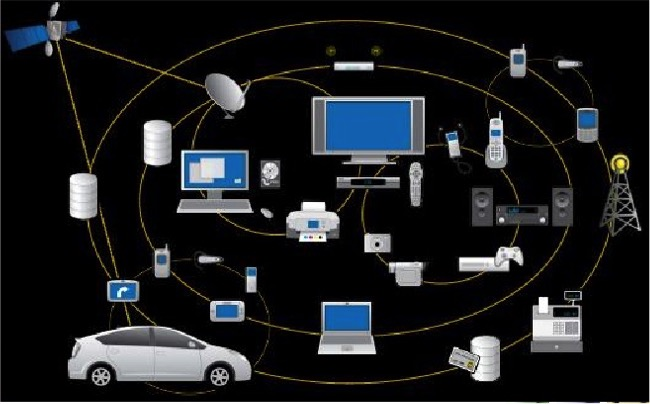
\includegraphics[scale=0.5]{img/everywhere}
\end{frame}

\begin{frame}
  \frametitle{Testes e Correção de Software}
	\begin{columns}[T]
		\begin{column}{.35\textwidth}
			\begin{tabular}{c}
				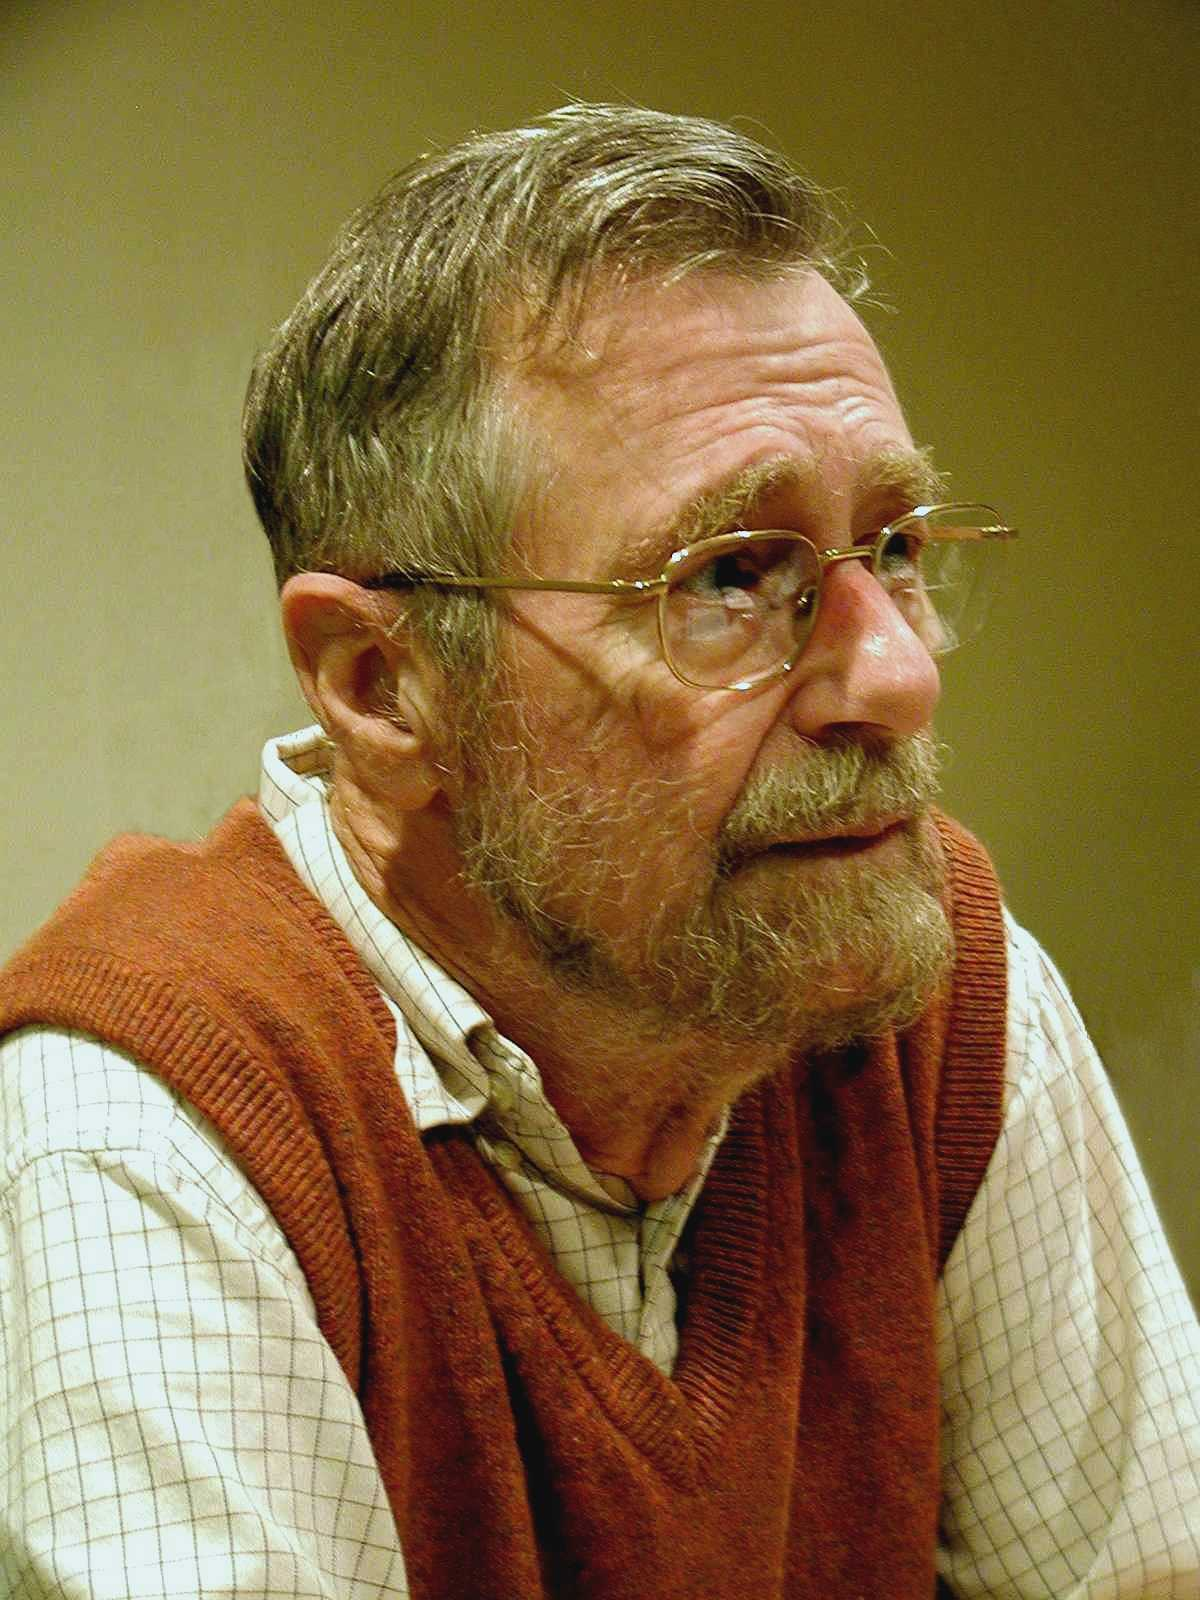
\includegraphics[scale=.1]{img/dijkstra.jpg} \\
			\end{tabular}
		\end{column}
		\begin{column}{.65\textwidth}
			\begin{quote}
				\justifying {\large{``Testing can only show the presence, not the absence of bugs.''}}
			\end{quote}
		\end{column}
	\end{columns}
\end{frame}

\begin{frame}
   \frametitle{Verificação Formal}
   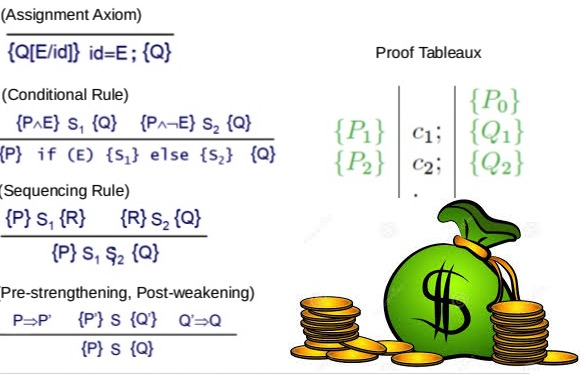
\includegraphics[scale=0.5]{img/hoarelogic}
\end{frame}

\begin{frame}
  \frametitle{Teoria de Tipos}
	\begin{columns}[T]
		\begin{column}{.5\textwidth}
                   \[
                        \begin{array}{c}
                        \infer[_{(TVar)}]{\Gamma\,\vdash\,x : \tau}
                                             {x: \sigma \in \Gamma &
                                                                     \tau
                                                                     \sqsubseteq
                                                                     \sigma}
                          \\ \\
                        \infer[_{(TApp)}]{\Gamma\,\vdash\,e\:e' :\tau}
                                             {\Gamma\,\vdash\,e :\tau'
                                               \to \tau &
                                              \Gamma\,\vdash\,e':\tau'}
                       \end{array}
                   \]
		\end{column}
		\begin{column}{.5\textwidth}
			\begin{quote}
				\justifying {\textbf{Testing} can
                                  prove the absence of bugs, if we
                                  reduce program's weirdness.}
			\end{quote}
		\end{column}
	\end{columns}
\end{frame}

\begin{frame}
  \frametitle{Pesquisa: Aplicações de Teoria de Tipos}
  \begin{itemize}
      \item Software correto por construção.
      \begin{itemize}
           \item Especificações expressas como tipos. Verificação de
             correção feita pelo compilador.
           \item Trabalhos realizados: Intepretadores, algoritmos e
             estruturas de dados.
           \item Em andamento: Sistemas de tipos para verificação de
             propriedades de sistemas embarcados.
      \end{itemize}
      \item Formalização
      \begin{itemize}
           \item Uso de assistentes de provas para demonstração de
            propriedades de formalismos como sistemas de tipos.
            \item Construção de provas de terminação de algoritmos sem
              efeitos colaterais em linguagens funcionais.
      \end{itemize}
  \end{itemize}
\end{frame}

\section{Modularização e Extensibilidade de Linguagens}

\begin{frame}
  \frametitle{Era da Produtividade}
%  \putat{200}{-10}{
\includegraphics[width=3.8cm]{img/efficiency_01}}
  \putat{200}{-10}{
\includegraphics[width=3.6cm]{img/focus}}
  \begin{itemize}
    \item Foco na eficiência do programador
    \item DSLs como uma alternativa para melhorar a eficiência do programador
    \item Linguagens extensíveis como mecanismo para implementar e usar DSLs
  \end{itemize}
  \putat{5}{-70}{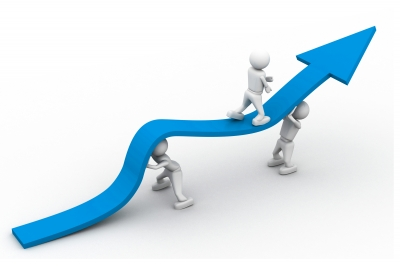
\includegraphics[width=3.5cm]{img/efficiency}}
\end{frame}

\begin{frame}[fragile]
  \frametitle{O que são Linguagens Extensíveis?}
  \begin{itemize}
    \item Linguagens extensíveis são linguagens que permitem estender a própria sintaxe concreta
  \end{itemize}
    \begin{columns}[!ht]
    \begin{column}{5.5cm}
\begin{lstlisting}[language=java,
                   frame=bottomline,title={SugarJ defining syntax}]
package syntactic;
public sugar Pair {
  context-free syntax
   "("JavaType "," JavaType")"
        $\rightarrow$ $\alert<1>{JavaType}$
   "("JavaExpr "," JavaExpr")"
        $\rightarrow$ $\alert<2>{JavaExpr}$
  ...
}
\end{lstlisting}
    \end{column}
    \begin{column}{5.5cm}
\begin{lstlisting}[language=java,frame=bottomline,title={Using Pair syntax},escapechar=\%]
import syntactic.Pair;
public class Test {
 private $\alert<1>{(String, Integer)}$ p
               = %\alert<2>{("12", 34)}%;
}
\end{lstlisting}
    \end{column}
  \end{columns}
\end{frame}

\defverbatim[colored]\sugarj{
    \begin{columns}[!ht]
    \begin{column}{5.5cm}
\begin{lstlisting}[language=java,
                   frame=bottomline,title={SugarJ defining syntax}]
package syntactic;
public sugar Pair {
  context-free syntax
   "("JavaType "," JavaType")"
        $\rightarrow$ JavaType
   "("JavaExpr "," JavaExpr")"
        $\rightarrow$ JavaExpr
  ...
}
\end{lstlisting}
    \end{column}
    \begin{column}{5.5cm}
\begin{lstlisting}[language=java,frame=bottomline,title={Using Pair syntax},escapechar=\%]
%\alert{import syntactic.Pair;}%
public class Test {
 private (String, Integer) p
               = ("12", 34);
}
\end{lstlisting}
    \end{column}
  \end{columns}
}

\begin{frame}[fragile]
  \frametitle{Como Essas Características Dinâmicas Afetam o Parsing?}
  \begin{itemize}
    \item Necessidade de modificar o parser de forma dinâmica, durante a análise da entrada
  \end{itemize}
  \sugarj
\end{frame}

\begin{frame}
  \frametitle{As Teorias de Parsing Suportam Modificação Dinâmica?}
  \begin{itemize}
    \item Principais avanços recentes na área não tratam de modificações dinâmicas
      \begin{itemize}
        \item PEG, LL(*), Adaptative LL(*), SGLR, YAKKER
      \end{itemize}
    \item Trabalhos que lidam com modificação dinâmica das regras têm eficiência questionável ou não apresentam algoritmos de parsing
      \begin{itemize}
        \item Adaptable Grammar de Christiansen; RAG; Parsing Reflective Grammars;
        \item AMG; Dynamic Grammars; Evolving Grammars
      \end{itemize}
  \end{itemize}
  %\hspace{9cm} 
\includegraphics[width=2.5cm]{img/question.jpg}
  \putat{270}{-60}{
\includegraphics[width=2.5cm]{img/question.jpg}}
\end{frame}

\begin{frame}[fragile]
  \frametitle{Adaptable Parsing Expression Grammars}
  \begin{itemize}
   \item Extensão de Parsing Expression Grammar;
   \item Modelo que permite modificações no conjunto de regras dinamicamente.
  \end{itemize}
  \putat{220}{45}{
\includegraphics[width=4cm]{img/efficiency_01}}
  \putat{10}{-100}{
\includegraphics[width=4cm]{img/camaleao}}
  \putat{220}{-90}{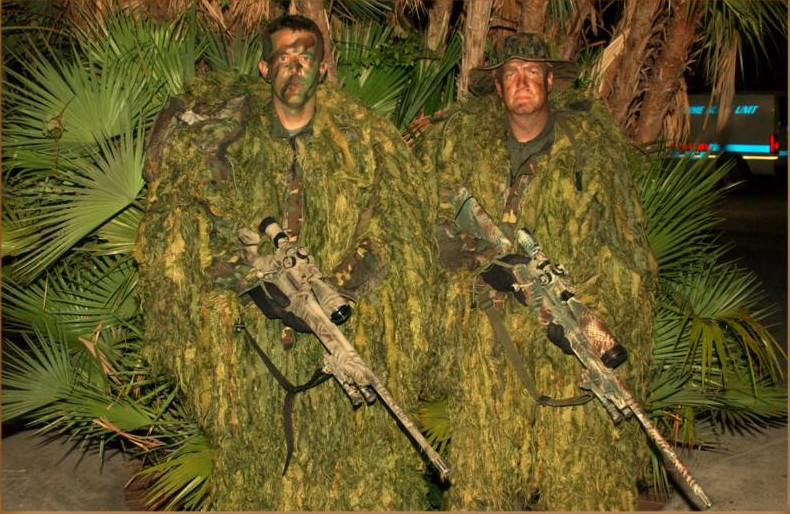
\includegraphics[width=4cm]{img/adapt}}
\end{frame}

\begin{frame}
 \frametitle{A Pesquisa}
 \begin{itemize}
  \item Desenvolvimento de um gerador automático de analisador sintático baseado em APEG:
   \begin{itemize}
    \item Implementação eficiente;
    \item Tratamento de erros;
    \item Construção automática de AST e metaprogramação;
    \item provas de propriedades;
   \end{itemize}
  \item Análise (métricas) de uso de DSLs em sistemas;
  \item Formalismos e mecanismos para especificação modular de linguagens
   \begin{itemize}
    \item o que é modularização no contexto de especificação de linguagens?
    \item especificação de sintaxe e semântica;
    \item implementação de DSLs como bibliotecas.
   \end{itemize}
 \end{itemize}
\end{frame}

\section{Elton'work}

\begin{frame}
 \frametitle{Espaço do Elton}
\end{frame}

%% GLAUBER
\section{Correção e Avaliação Automáticas em Sistemas MOOCs}

\begin{frame}
  \frametitle{MOOCs}

  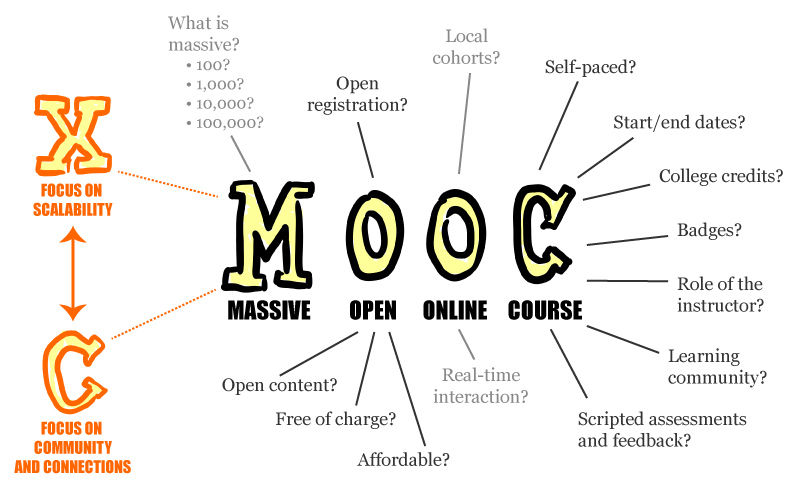
\includegraphics[scale=0.4]{img/moocs.jpg}
\end{frame}

\begin{frame}
 \frametitle{Correção Automáticas de Programas em MOOCs}

  \begin{block}{Correção Automática}
    \begin{itemize}
      \item Suporte a linguagens funcionais: \textit{Haskell}, \textit{Scala}, \ldots
      \item Geração de valores de teste automaticamente
      \item Sistemas atuais: testes caixa preta
      \item É preciso fornecer melhor retorno dos erros aos alunos!
    \end{itemize}
  \end{block}

  \begin{center}
    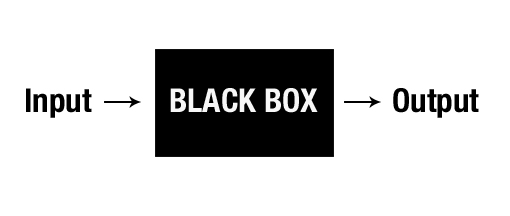
\includegraphics[scale=0.4]{img/blackbox.jpg}
  \end{center}

\end{frame}

\begin{frame}
 \frametitle{Avaliação Automáticas de Programas em MOOCs}

    \begin{block}{Avaliação Automática}
      \begin{itemize}
        \item Retorno indicativo dos erros no código
        \item Sugestões de alterações para corrigir o código
        \item Medir progresso do estudante
      \end{itemize}
    \end{block}

    \begin{center}
      
\includegraphics[scale=0.3]{img/duvida.jpg}
      \hspace{1cm}
      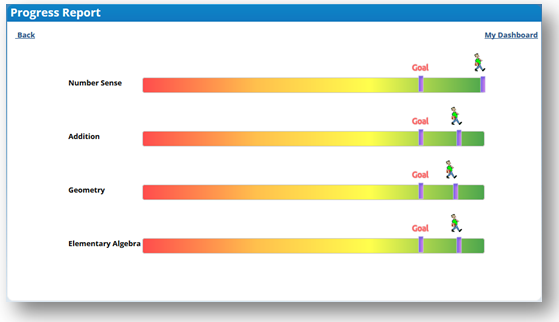
\includegraphics[scale=0.3]{img/progresso.png}
    \end{center}
\end{frame}

\begin{frame}[fragile]
  \frametitle{Pesquisa}

  \begin{columns}[T]
    \begin{column}{.35\textwidth}
      \begin{tabular}{c}
        
\includegraphics[scale=0.1]{img/pesquisa.jpg}
      \end{tabular}
    \end{column}
    
    \begin{column}{.65\textwidth}

      \begin{itemize}
        \item Desenvolver ou adaptar sistema para linguagens funcionais
        \item Gerar valores de testes com testes automatizados
        \item Gerar retorno de erros com base no sistema de tipos
        \item Adaptar avaliação de progresso para linguagens funcionais
      \end{itemize}

    \end{column}
  \end{columns}
\end{frame}

\end{document}
